%versi 2 (8-10-2016)
\chapter{Landasan Teori}
\label{chap:teori}


Pada bab ini akan berisi landasan-landasan teori yang dipakai pada penelitian ini.

\section{Code Igniter}
\label{sec:codeigniter}


CodeIgniter\cite{codeigniter3} adalah \textit{framework} untuk pembuat website yang menggunakan \textit{PHP}. \textit{CodeIgniter} mempermudah \textit{developer} untuk meminimalisir penggunaan kode untuk mengakses suatu fungsi. Seperti untuk mengambil data pada \textit{database}, mengakses file \textit{php} lainnya. Penggunaan \textit{framework CodeIgniter} juga mudah.\textit{ Developer} tidak perlu melakukan banyak konfigurasi--konfigurasi saat melakukan \textit{setup}.\textit{CodeIgniter} juga memberikan dokumentasi yang lengkap. Permasalahan \textit{routing}  sudah diselesaikan oleh \textit{framework} ini. \textit{ Framework} ini secara otomatis akan mengarah ke file dalam \textit{directory controllers} sesuai dengan \textit{path-abempty} pada \textit{URI}  dan menjalankan \textit{method} \texttt{index()}.


\begin{figure}[H]
	\centering
	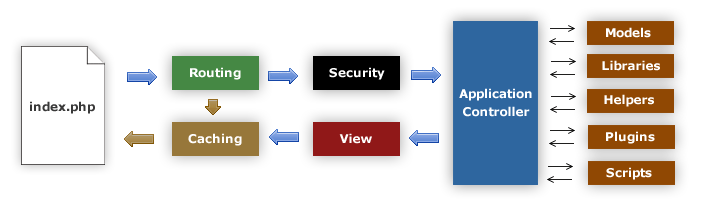
\includegraphics[scale=0.8]{mvc} 
	\caption{Flowchart MVC}
	\label{fig:appflowchart} 
\end{figure}


\textit{CodeIgniter} menerapkan arsitektur \textit{MVC} yang dapat dilihat pada gambar \ref{fig:appflowchart}, file \texttt{index.php} berfungsi mengatur routing dan mengarahkan ke \textit{application controller} yang berada di \textit{directory controller} dan melalui \textit{controller} akan dipanggil \textit{models, libraries, helpers, etc} yang dibutuhkan dengan perintah \texttt{\$this->load-><<apa\_yang\_mau\_diload>>(\lq<<nama\_file>>\rq)}. Masukan akan diolah melalui \textit{models} dan hasil yang sudah siap akan dikirim ke \textit{view} melalui \textit{controller}. Fitur tambahan dari arsitektur \textit{CodeIgniter} adalah saat \textit{router} memeriksa \textit{HTTP request} jika \textit{cache} tersedia maka akan dikirimkan \textit{cache} tersebut dan jika tidak ada \textit{cache} maka \textit{security} akan memeriksa dan melakukan filter terhadap \textit{HTTP request} seperti pada gambar \ref{fig:appflowchart}. 

\subsection{Controller}

\textit{Controller} adalah pusat dari aplikasi, \textit{controller} menangani apa yang harus dilakukan dari \textit{HTTP request}. Dalam CodeIgniter untuk menginisiasi \textit{controller} cukup menulis nama kelas diikuti dengan \texttt{extends CI\_Controller} sebagai contoh:

\begin{lstlisting}
<?php
defined('BASEPATH') OR exit('No direct script access allowed');
		
class Welcome extends CI_Controller {

	public function index()
	{
		$this->load->view('welcome_message');
	}
}
\end{lstlisting}

\textit{CodeIgniter} secara otomatis akan menjalankan \textit{method} \texttt{index()} jika tidak diperintahkan untuk menjalankan \textit{method} tertentu. Untuk menjalankan \textit{method} lain hanya perlu ditambahkan \textit{path-abempty} seperti  \texttt{example.com/index.php/Welcome/<<nama\_method>>}.
fungsi diatas akan mengembalikan file \textit{welcome\_message.php} pada direktori \textit{view}. Developer dapat menaruh parameter pada \textit{view} tersebut.

\begin{lstlisting}
<?php
defined('BASEPATH') OR exit('No direct script access allowed');
	
class Welcome extends CI_Controller {
	
	public function __construct(){
		parent::_construct();
		$this->load->database();
		$this->load->model(contoh_model);
	}
	
	public function index()
	{
		$t = "hello";
		$this->load->view('welcome_message',array(
		't' => $t));
	}
}
\end{lstlisting}


Fungsi \textit{constructor} yang dijalankan pada \textit{codeigniter} harus memanggil \texttt{parent::construct()}. Dalam contoh diatas juga dapat dilakukan \textit{load model} dan \textit{database}. File \textit{model} akan berada di direktori \textit{model} sedangkan untuk \texttt{\$this->load->database()} akan melakukan \textit{load} pada \textit{database} menggunakan parameter yang ada di direktori \texttt{/config/database.php}. Begitu juga dengan kebutuhan--kebutuhan lainnya dapat dilakukan dengan \textit{method} \texttt{\$this->load}.


\subsection{Model}

\textit{Model} berfungsi sebagai \textit{logic} dari aplikasi. \textit{ Model} pada \textit{CodeIgniter} bersifat opsional, tetapi disediakan untuk \textit{developer} yang ingin menggunakan MVC\cite{codeigniter3}. 

\begin{lstlisting}
class Blog_model extends CI_Model {

	public $title;
	public $content;
	public $date;
	
	public function get_last_ten_entries()
	{
		$query = $this->db->get('entries', 10);
		return $query->result();
	}
}
\end{lstlisting}

\textit{Model} pada \textit{CodeIgniter} harus diikuti dengan \texttt{extends CI\_Model}. Hal yang berurusan terhadap \textit{database} dapat dilakukan dengan perintah \texttt{\$this->db->query(\lq<<isi query>>\rq)} atau untuk mempermudah, beberapa fungsi \textit{MYSQL} dasar disediakan oleh \textit{CodeIgniter}.\textit{ Method} bisa langsung digunakan seperti \texttt{\$this->db->get(\lq<<nama tabel>>\rq)}
untuk mengambil semua nilai dari tabel tersebut. Untuk dapat mengakses \textit{database} maka harus dipasang \textit{database} yang akan digunakan pada \texttt{config/database.php}.

\begin{lstlisting}
		
$config['hostname'] = 'localhost';
$config['username'] = 'myusername';
$config['password'] = 'mypassword';
$config['database'] = 'mydatabase';
$config['dbdriver'] = 'mysqli';
$config['dbprefix'] = '';
$config['pconnect'] = FALSE;
$config['db_debug'] = TRUE;

$this->load->model('model_name', '', $config);
\end{lstlisting}

File \texttt{database.php} diatas menyimpan kredensial dari \textit{database} yang digunakan. Mulai dari \textit{hostname, username, password, dst}.

\subsection{View}


\textit{View} tidak pernah dipanggil secara langsung, \textit{view} harus dipanggil melalui \textit{controller}\cite{codeigniter3}.
\textit{View} pada \textit{CodeIgniter} ditaruh pada direktori \textit{view}. Pemanggilan \textit{view} menggunakan \textit{method} 
\begin{lstlisting}
$this->load->view('nama_view');
\end{lstlisting}

Jika \textit{controller} ingin mengirimkan data kepada \textit{view} maka perlu dilakukan 

\begin{lstlisting}
$t = "hello";
$this->load->view('welcome_message',array(
't' => $t));
\end{lstlisting}

Selanjutnya untuk menampilkan data tersebut ke halaman
 
\begin{lstlisting}
html>
<head>
</head>
<body>
	<h1><?php echo $t ?></h1>
</body>
</html>
\end{lstlisting}


\section{Phpspreadsheet}
\label{section:phpspreadsheet}

\begin{table}[H]
	\centering
	\begin{tabular}{|p{0.5\textwidth}|c|c|}
		\hline
		\textbf{Format} & \textbf{Reading} & \textbf{Writing} \\ \hline
		Open Document Format/OASIS (.ods) & \checkmark & \checkmark \\ \hline
		Office Open XML (.xlsx) Excel 2007 and above & \checkmark & \checkmark \\ \hline
		BIFF 8 (.xls) Excel 97 and above & \checkmark & \checkmark \\ \hline
		BIFF 5 (.xls) Excel 95 & \checkmark  & \\ \hline
		SpreadsheetML (.xml) Excel 2003 & \checkmark & \\ \hline
		Gnumeric & \checkmark & \\ \hline
		HTML & \checkmark & \checkmark \\ \hline
		SYLK & \checkmark & \\ \hline
		CSV & \checkmark & \checkmark \\ \hline
		PDF (using either the TCPDF, Dompdf or mPDF libraries, which need to be installed separately) & & \checkmark \\ 
		\hline
	\end{tabular}
\caption{Tabel format yang didukung oleh phpspreadsheet}
\label{tab:phpspreadsheet supported}
\end{table}


PhpSpreadsheet adalah \textit{library} yang ditulis dengan bahasa PHP berguna untuk membaca dan menulis file dengan jenis spreadsheet seperti Excel dan LibreOffice Calc\cite{phpspreadsheet}. Format--format yang didukung oleh phpspreadsheet dapat dilihat pada tabel \ref{tab:phpspreadsheet supported}. Pada penelitian kali ini phpspreadsheet hanya digunakan untuk menulis ke dokumen dengan \textit{extension} \texttt{.xls}

\subsection{Instalasi Phpspreadsheet}
Sebelum dapat menginstalasi phpspreadsheet dibutuhkan composer. Composer dapat diunduh pada \url{getcomposer.org}. dan menjalankan perintah:

\begin{lstlisting}
composer require phpoffice/phpspreadsheet
\end{lstlisting}

Masukkan perintah tersebut untuk membuat file \texttt{composer.json} dan menginstalasi \textit{dependencies} tersebut. Contoh untuk menggunakan phpspreadsheet dapat dilihat sebagai berikut:

\begin{lstlisting}
<?php

require 'vendor/autoload.php';

use PhpOffice\PhpSpreadsheet\Spreadsheet;

$spreadsheet = new Spreadsheet();
$sheet = $spreadsheet->getActiveSheet();
\end{lstlisting}

Penggunaan phpspreadsheet secara dasar membutuhkan perintah \texttt{use PhpOffice$\backslash$PhpSpread-\\-sheet$\backslash$Spreadsheet} dan \texttt{new Spreadsheet()}. Untuk menrubah, menambah atau mengganti isi dari suatu kolom dibutuhkan \textit{method} \texttt{getActiveSheet()}.

\subsection{Menempatkan Nilai pada Kolom tertentu}

\textit{Phpspreadsheet} menyediakan suatu \textit{method} untuk dapat menaruh atau merubah \textit{value} pada cell tertentu

\begin{lstlisting}
$sheet->setCellValue('A1', 'PhpSpreadsheet');
\end{lstlisting}

 Fungsi diatas akan menulis \lq PhpSpreadsheet \rq pada kolom \lq A1 \rq .

\begin{lstlisting}
$sheet->getStyle('A1')->getFont()->setBold(true);
\end{lstlisting}

 \textit{Method} diatas dapat digunakan untuk membuat nilai pada kolom \lq A1\rq menjadi \textit{bold}.

\begin{lstlisting}
$arrayData = [
	[NULL, 2010, 2011, 2012],
	['Q1',   12,   15,   21],
	['Q2',   56,   73,   86],
	['Q3',   52,   61,   69],
	['Q4',   30,   32,    0],
];
$spreadsheet->getActiveSheet()
	->fromArray(
		$arrayData,  
		NULL,        
		'C3'         
	);
\end{lstlisting}

\textit{Phpspreadsheet} menyediakan \textit{method} \texttt{fromArray} yang dapat menerima masukan berupa \textit{array} 2 dimensi. \texttt{fromArray} menerima 3 parameter. Parameter pertama berupa data dari \textit{array} tersebut, parameter kedua adalah \textit{value} yang tidak akan di set pada \textit{spreadsheet} dan parameter ketiga adalah lokasi dimana \textit{array} akan ditaruh. Secara \textit{default} parameter kedua berisi \textit{NULL} dan parameter ketiga berisi \texttt{A1}. 

\subsection{Menulis Spreadsheet ke Xls }

\textit{Phpspreadsheet} dapat melakukan \textit{read and write} ke banyak format. Mulai dari \textit{xls,xlsx,csv} dll. Pada kali ini format yang akan digunakan adalah \textit{xls}.

\begin{lstlisting}
$writer = new \PhpOffice\PhpSpreadsheet\Writer\Xls($spreadsheet);
$writer->save("05featuredemo.xls");
\end{lstlisting}

Penggunaan fungsi \textit{write} dari \textit{phpspreadsheet} membutuhkan kelas \texttt{\textbackslash PhpOffice\textbackslash PhpSpread-\\-sheet\textbackslash Writer\textbackslash Xls()}. Kelas lain yang dapat digunakan untuk \textit{read}\&\textit{write} adalah \texttt{\textbackslash PhpOffice\textbackslash\\ PhpSpreadsheet\textbackslash IOFactory::createWriter(\$ spreadsheet, "Xlsx")}

\section{Bootstrap}



 
